
% Copyright (c) 2008, João Henrique Ferreira de Freitas
% All rights reserved.
% 
% Redistribution and use in source and binary forms, with or without modification,
% are permitted provided that the following conditions are met:
% 
%     * Redistributions of source code must retain the above copyright notice,
%       this list of conditions and the following disclaimer.
%     * Redistributions in binary form must reproduce the above copyright notice,
%       this list of conditions and the following disclaimer in the documentation and/or 
%       other materials provided with the distribution.
%     * Neither the name of the <ORGANIZATION> nor the names of its contributors may
%       be used to endorse or promote products derived from this software without 
%       specific prior written permission.
% 
% THIS SOFTWARE IS PROVIDED BY THE COPYRIGHT HOLDERS AND CONTRIBUTORS "AS IS" AND ANY 
% EXPRESS OR IMPLIED WARRANTIES, INCLUDING, BUT NOT LIMITED TO, THE IMPLIED WARRANTIES
% OF MERCHANTABILITY AND FITNESS FOR A PARTICULAR PURPOSE ARE DISCLAIMED. IN NO EVENT
% SHALL THE COPYRIGHT OWNER OR CONTRIBUTORS BE LIABLE FOR ANY DIRECT, INDIRECT, INCIDENTAL,
% SPECIAL, EXEMPLARY, OR CONSEQUENTIAL DAMAGES (INCLUDING, BUT NOT LIMITED TO, PROCUREMENT
% OF SUBSTITUTE GOODS OR SERVICES; LOSS OF USE, DATA, OR PROFITS; OR BUSINESS INTERRUPTION)
% HOWEVER CAUSED AND ON ANY THEORY OF LIABILITY, WHETHER IN CONTRACT, STRICT LIABILITY,
% OR TORT (INCLUDING NEGLIGENCE OR OTHERWISE) ARISING IN ANY WAY OUT OF THE USE OF THIS
% SOFTWARE, EVEN IF ADVISED OF THE POSSIBILITY OF SUCH DAMAGE.
% 
% $Id$

\section{Anexo E: Detalhes da implementação} \label{sec:anexoe}

\subsection{Sobre o Bacula}
Bacula é um conjunto de softwares (vide figura \ref{fig:arqbacula}) no qual permitem gerenciar \textit{backups}, \textit{restores} e verificações através da rede de diversos tipos de computadores. Bacula é relativamente fácil de usar e eficiente, oferece muitos meios de armazenar os dados e recursos para gerenciá-los, procurá-los e recuperá-los. A maioria do código fonte está licenciada sob a licença GPL versão 2 e com direitos passados para a Free Software Foundation Europa.

\subsection{Introdução}
Como podemos notar na figura \ref{fig:arqbacula} o software Bacula possui um conjunto de programas nos podem ser instalados e executados em diferentes máquinas dentro de uma rede.
Os principais componentes são:
\begin{itemize}
\item Servidor de Backup, denominado de \textit{bacula-dir}, com as funções de orquestrar toda a solução;
\item Servidor de Armazenamento, denominado de \textit{bacula-sd}, responsável por armazenar todos os arquivos enviados pelos bacula-fd;
\item Servidor de Arquivos, denomindado de \textit{bacula-fd}, responsável por enviar para o bacula-sd os arquivos necessários para serem armazenados provenientes dos computadores de uma rede;
\item Estações de Administração, denomindas de \textit{console}, são utilizadas para controlar via linha de comando ou interface gráfica as operações e tarefas do Bacula;
\item Servidor de Banco de Dados, denominado \textit{catalog database} ou banco de dados, armazena os meta-dados (características de cada arquivo).
\end{itemize}

\begin{figure}[h]
 \centering
 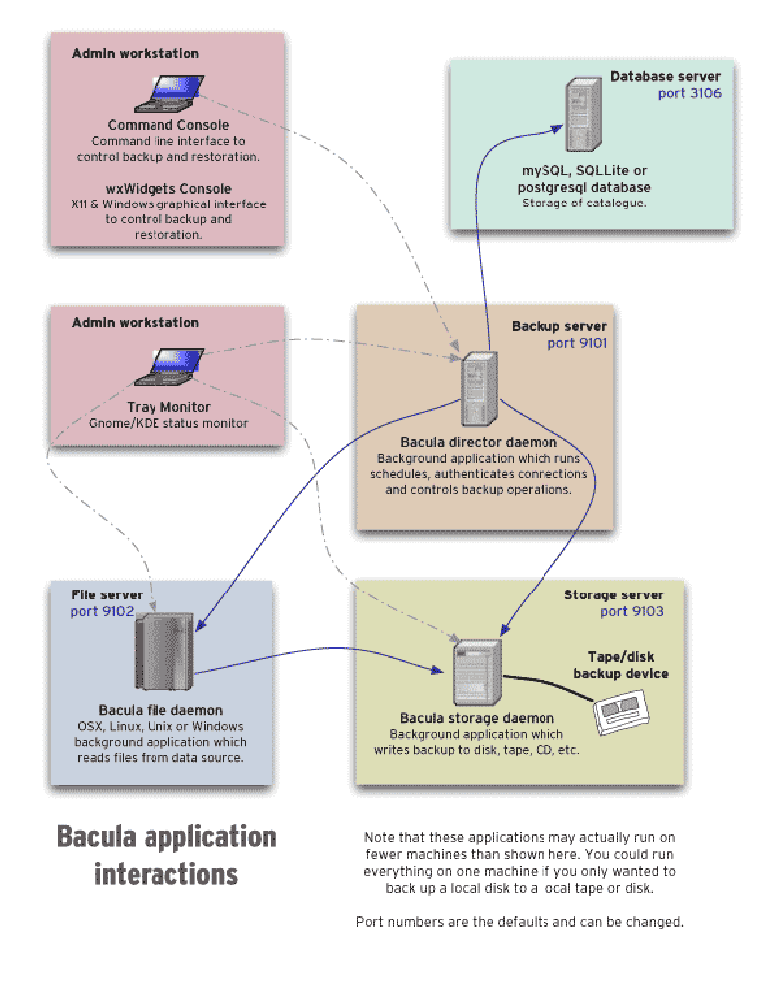
\includegraphics[scale=0.8]{../../doc/figuras/bacula-applications.eps}
 % bacula-applications.png: 1179666x1179666 pixel, 0dpi, infxinf cm, bb=
 \caption[Arquitetura geral do Bacula]{Arquitetura geral do sistema \\ \url{http://www.bacula.org/en/dev-manual/What_is_Bacula.html}}
 \label{fig:arqbacula}
\end{figure}

Durante a implementação do patch \patchshort, concentramos apenas nos componentes bacula-dir e catalog database. Não tivemos a necessidade de interferir nos outros componentes do sistema pois tratavam operações nas quais não nos interessavam no momento.

Para ajudar no entendimento, a figura \ref{fig:comparativo} oferece uma visão geral  antes e depois da implementação do patch. 

Na figura \ref{fig:unico} notamos a utilização de um único banco de dados por binário, ou seja, a escolha de qual banco de dados utilizado é definida durante a compilação do código fonte do Bacula, no qual eram definidos os códigos necessários para construir o driver de acesso nativo via API própria de cada banco de dados. A camada sql\_\*.c utiliza as funções definidas em [banco de dados].c,  onde [banco de dados] pode ser apenas um dentre: mysql, postgresql, sqlite. Desta forma, uma vez compilado, o usuário apenas utilizaria o banco de dados escolhido. 
Um outro ponto é o suporte aos bancos de dados limitados, ou seja, apenas para os SGBDs codificados no Bacula.

Já na figura \ref{fig:dbi} observamos um novo cenário no qual uma camada de abstração (via bibliotema libdbi) e um driver (dbi.c) para fazer a interface entre a camada sql\_\*.c e a libdbi foi implementado. Basicamente para garantir dois pontos: 
\begin{itemize}
\item O primeiro é a independência do banco de dados a ser utilizado pelo Bacula. 
\item O segundo ponto é a possibilidade de utilizar vários tipos de SGBDs para armazenar meta-dados de arquivos.                                                                   \end{itemize}
Um exemplo do segundo ponto abordado é a possibilidade de realizar backups entre bancos de dados ou até mesmo a transferência de um catálogo de um banco de dados para outro completamente distinto em caso de problemas ou manutenções.

\begin{figure*}[h]
 \centerline{
  \subfigure[Único banco de dados por binário]{
  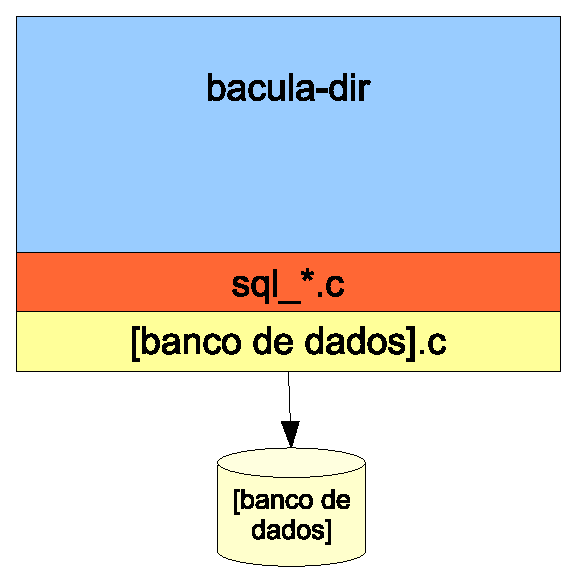
\includegraphics[width=5cm]{../../doc/diagramas/bacula-dir-sgbd.eps}
  \label{fig:unico}
  }
  \hfil
  \subfigure[Vários tipos de banco de dados por binário]{
  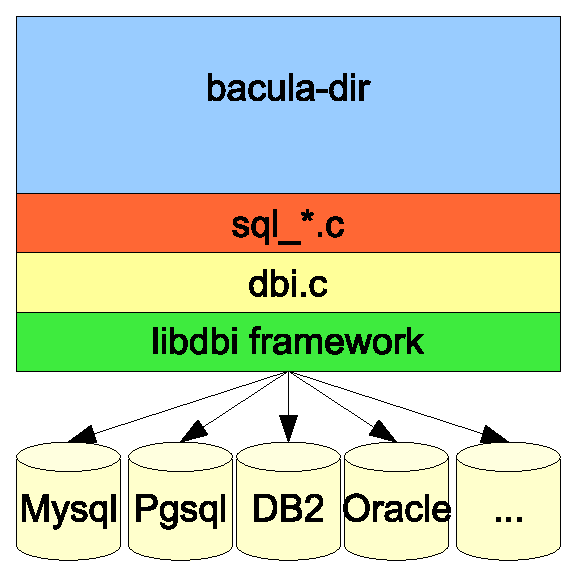
\includegraphics[width=5cm]{../../doc/diagramas/bacula-dir-dbi.eps}
  \label{fig:dbi}
  }
 } 
 \label{fig:comparativo}
 \caption[Comparativo de implementação]{Comparativo da implementação realizada \subref{fig:unico} e \subref{fig:dbi}}
\end{figure*}

\subsection{Limitações}

A principal limitação encontrada é referente a existência de diversos tipos de SGBDs utilizando diferentes dialetos e recursos da linguagem SQL. Não é possível prever todos os casos. Há consultas que funcionam em todos os SGBDs e outras que são específicas e devem ser tratadas a parte. 

A biblioteca libdbi oferece uma abstração para os diferentes tipos de APIs de cada fabricante de SGBDs mas a mesma não oferece nenhum suporte aos diferentes tipos de SQL utilizados por eles.

Sendo assim o Bacula deve ser preparado para suportar os diferentes dialetos SQL, ou seja, para cada banco de dados temos um conjunto de SQL que devem ser adptadas e suportadas para que o SGBD seja efetivamente suportado. Isso se torna uma limitação pois necessita de uma intervenção no código para o correto funcionamento.

\subsection{Implementação}

As tarefas de criação do ambiente necessário para a implementação e definição de quais arquivos seriam necessários criar ou alterar não foram complicadas. Notamos um software bem modularizado e dividido para facilitar a manutenção e adiçaõ de novos recursos. A seguir apresentamos uma macro lista dos itens no qual foram necessário trabalhar:

\begin{itemize}
\item Alteração no arquivo \url{src/cats/cats.h}: 
 \subitem inclusão da regra de compilação condicional HAVE\_DBI para o compilador reconhecer o código para o driver DBI
 \subitem adaptado a estrutura de dados B\_DB, responsável pelo gerenciamento de todos os itentes relacionados a banco de dados, dentro do Bacula, bem como as definições de várias funções para a API da libdbi
\item Alteração dos arquivos \url{src/cats/sql*.c}: incluindo a regra de compilação condicional HAVE\_DBI
\item Criado o arquivo \url{src/cats/dbi.c} baseado no código \url{src/cats/postgresql.c}
 \subitem tranformado e convertigo as funções presentes no arquivo src/cats/dbi.c de um código com APIs referentes ao SGBD postgresql para APIs da  biblioteca DBI. Evidente que muitas funções presentes no SGBD postgresql não seguiam a mesma lógica utilizada na biblioteca DBI. Sendo necessário estudar as documentações e códigos de ambas para entender o funcionamento e decidir se a API da biblioteca DBI atendia ou não a forma na qual o Bacula estava projetado para interagir com um SGBD. 
\item Alterado o arquivo \url{src/dird/dird_conf.h} e \url{src/dird/dird_conf.c}
 \subitem adicionado a opção de configuração dbdriver no qual informava ao Bacula qual driver e banco de dados será utilizado.
\item Alterado os arquivos \url{src/autoconf/config.h.in} e \url{src/autoconf/bacula-macros/db.m4} referentes a geração do script de autoconfiguração para compilação, baseados nas disponibilidades dos requisitos da plataforma.
\item Adaptação de todos os testes de regressão para incluir as opções de configuração para o driver DBI
\end{itemize}

\subsection{Timeline do desenvolvimento}
\begin{table}[htbp]
\begin{tabular}{|l|c|c|c|c|}
\hline
 & \textbf{Data} & \textbf{Submissões} & \textbf{Data Integração} & \textbf{Revision} \\ \hline
\multicolumn{ 1}{|c|}{\textbf{Exploração Arquitetural}} & 2007-12-07 &  &  &  \\ \cline{ 2- 5}
\multicolumn{ 1}{|l|}{} & 2008-01-11 &  &  &  \\ \hline
\multicolumn{ 1}{|c|}{\textbf{Desenvolvimento}} & 2008-01-18 &  &  &  \\ \cline{ 2- 5}
\multicolumn{ 1}{|l|}{} &  & 2008-02-01 & 2008-02-02 & 6358 \\ \cline{ 2- 5}
\multicolumn{ 1}{|l|}{} &  & 2008-02-12 & 2008-02-13 & 6413 \\ \cline{ 2- 5}
\multicolumn{ 1}{|l|}{} &  & 2008-02-19 & 2008-02-22 & 6464 \\ \cline{ 2- 5}
\multicolumn{ 1}{|l|}{} &  & 2008-02-21 & 2008-02-27 & 6498 \\ \cline{ 2- 5}
\multicolumn{ 1}{|l|}{} &  & 2008-02-25 & 2008-04-15 & 6825 \\ \cline{ 2- 5}
\multicolumn{ 1}{|l|}{} &  & 2008-03-17 & 2008-04-15 & 6826 \\ \cline{ 2- 5}
\multicolumn{ 1}{|l|}{} &  & 2008-04-09 & 2008-04-09 & 6817 \\ \cline{ 2- 5}
\multicolumn{ 1}{|l|}{} &  & 2008-04-14 & 2008-04-15 & 6818 \\ \cline{ 2- 5}
\multicolumn{ 1}{|l|}{} &  & 2008-04-27 & 2008-04-27 & 6874 \\ \cline{ 2- 5}
\multicolumn{ 1}{|l|}{} & 2008-05-02 &  &  &  \\ \hline
 &  &  &  &  \\ \hline
 & \textbf{Orçadas} & \textbf{Trabalhadas} &  &  \\ \hline
\textbf{Exploração Arquitetural:} & 64h & 59.89h &  &  \\ \hline
\textbf{Desenvolvimento:} & 168h & 118h &  &  \\ \hline
\end{tabular}
\caption{Timeline}
\label{Timeline}
\end{table}
